% !TEX root = main.tex
\documentclass{article}

\usepackage{neurips_2025}
\usepackage[utf8]{inputenc}
\usepackage[T1]{fontenc}
\usepackage{amsmath}
\usepackage{booktabs}
\usepackage{tabularx}
\usepackage{array}
\usepackage{xcolor}
\usepackage{graphicx}
\usepackage{url}
\usepackage{hyperref}

\newcolumntype{Y}{>{\raggedright\arraybackslash}X}
\newcolumntype{R}{>{\raggedleft\arraybackslash}p{0.12\linewidth}}
\newcommand{\artifact}[1]{\texttt{#1}}
\newcommand{\methodname}{PaperMemory}

\title{PaperMemory: Evidence-Packet Retrieval for Local-First Literature Assistance}

\author{Anonymous Author(s)}

\begin{document}

\maketitle

\begin{abstract}
PDF-based literature work can be slow because researchers need page-level evidence, citation support, and visible uncertainty before they can trust a draft answer. PaperMemory is a local-first compound AI assistant for postgraduate researchers who work with bounded PDF collections. It builds page-level EvidencePackets, combines visual and selectable-text retrieval, runs a bounded evidence-seeking loop, checks reliability, and keeps human verification in the workflow. Early market evidence from informal interviews with 10 PhD, master's, or postgraduate researchers gives a mean conditional purchase likelihood of 4.2/5 if the claimed functions are delivered, and 70\% prefer PaperMemory-provided API/model access through a monthly subscription rather than BYOK-only setup. We therefore evaluate a freemium model with a free BYOK tier and proposed 10 and 20~USD/month tiers that include weekly capped, provider-compliant API relay for managed LLM access. On the local synthetic fixture suite, BM25 improves Recall@1 from 77.8\% to 88.9\% and retrieval-level refusal correctness from 33.3\% to 100.0\%; robustness fixtures cover missing evidence, citation drift, prompt-injection-like PDF text, conflicts, and low-text pages. A cost stress test estimates positive base-case net savings for first-pass evidence gathering under stated assumptions, while leaving conversion, retention, hosting cost, support cost, licensing, and real-corpus retrieval quality as open commercialization risks.
\end{abstract}

\section{Introduction}

Postgraduate researchers often spend early writing time turning PDFs into claims they can safely cite. The hard part goes beyond finding a relevant page. A useful research assistant must show why a page was used, which citation supports the sentence, and where the answer should stop because the evidence is thin. When that boundary is hidden, users still have to redo the evidence work by hand.

PaperMemory targets this paid workflow directly. In informal interviews with 10 university PhD, master's, or postgraduate researchers, the mean conditional purchase likelihood was 4.2/5 if PaperMemory delivered the promised functions: local PDF ingestion, evidence-backed answers, visible citations, bounded uncertainty, and a simpler model-access path. Seven of the 10 interviewees preferred PaperMemory-provided API/model access through a monthly subscription over a BYOK-only setup \citep{paperMemoryInterviewValidation}. Appendix~\ref{app:interview-validation} records the short questionnaire protocol and aggregate response framing. This is early willingness-to-pay evidence, not product-market fit, but it is enough to justify testing a paid model in this course-stage report.

Existing research assistants such as Elicit and Consensus are priced around evidence-oriented workflows, although they are market comparators rather than executable baselines for this report \citep{elicitPricing,consensusPricing}. PaperMemory's narrower position is local-first PDF work: the user brings a scoped collection, the system builds page-level EvidencePackets, and the interface exposes citations, limits, and reliability status before the user turns the draft into research writing.

\begin{table}[t]
  \caption{A small postgraduate interview sample supports paid workflow interest, especially when PaperMemory provides managed model access, but the signal is early intent evidence.}
  \label{tab:market-validation}
  \centering
  \small
  \setlength{\tabcolsep}{4pt}
  \begin{tabularx}{\linewidth}{p{0.26\linewidth}p{0.18\linewidth}Y}
    \toprule
    Evidence item & Result & Boundary \\
    \midrule
    Interview sample & 10 postgraduate interviewees & Small interview sample, not a representative survey. \\
    Conditional purchase likelihood & 4.2 / 5 mean & Applies only if the claimed PDF, evidence, citation, and uncertainty workflow is delivered. \\
    API/model access preference & 70\% & Preference for product-provided API/model access through monthly subscription over BYOK-only setup. \\
    Proposed packaging & Free BYOK plus 10 and 20~USD/month tiers & Proposed revenue design, not actual conversion, retention, or production revenue. \\
    \bottomrule
  \end{tabularx}
\end{table}

\begin{table}[t]
  \caption{Major report claims and supporting evidence.}
  \label{tab:claim-evidence-boundary}
  \centering
  \small
  \setlength{\tabcolsep}{3pt}
  \begin{tabularx}{\linewidth}{p{0.32\linewidth}Y}
    \toprule
    Claim & Evidence in this report \\
    \midrule
    Market signal for a paid postgraduate workflow. & Interview aggregate: n=10 postgraduate researchers, 4.2/5 conditional purchase likelihood, and 70\% managed-access preference. \\
    PaperMemory is a compound AI system rather than a chat-only UI. & EvidencePackets, visual and text retrieval paths, BM25, hybrid page fusion, bounded evidence loop, reliability status, and evidence-visible UI. \\
    Retrieval components work on the local fixture suite. & Keyword, visual API, BM25, and hybrid rows; BM25 reaches 88.9\% R@1 and 100.0\% retrieval-level refusal correctness. \\
    Subscription packaging has bounded cost logic. & 10-PDF/30-PDF cost stress test plus provider-compliant API relay sensitivity. \\
    Trust behavior is implemented as visible limits. & Robustness matrix, failure gallery, reliability labels, citation filtering, and prompt-injection-like PDF text handling. \\
    \bottomrule
  \end{tabularx}
\end{table}


The contribution is both technical and commercial. Technically, PaperMemory combines page rendering, selectable-text manifests, BM25 retrieval, page-canonical rank fusion, EvidencePacket validation, bounded evidence seeking, reliability checks, and an evidence-visible UI. Commercially, it connects that workflow to a freemium BYOK product and proposed paid tiers that remove API setup friction through compliant managed model access. The evaluation remains bounded: synthetic/local metrics and controlled live tests show implementation behavior, not broad scholarly-corpus superiority.

\section{Product Boundary and Revenue Logic}

The first target users are postgraduate researchers who work with dense PDF collections and need a faster first pass over evidence. A second group is small research, consulting, or R\&D teams that need traceable evidence packets before writing memos or reports. PaperMemory is not a systematic-review replacement or final expert adjudicator. It supports evidence gathering, citation packaging, and uncertainty surfacing before human review.

The proposed packaging follows the interview signal. The free tier is BYOK with limited groups, which lowers adoption friction and keeps model cost outside the product. The 10~USD/month tier adds provider-compliant API relay for managed LLM access with a lower weekly managed-model boundary for routine postgraduate work. The 20~USD/month tier offers a larger workspace and a higher weekly managed-model boundary for heavier literature projects. The paid design assumes commercial API access or equivalent provider permission; it does not rely on consumer-account pooling, coding-plan resale, or unlimited inference. The exact quotas should be set only after usage telemetry exists; this report intentionally does not invent them.

\begin{table}[t]
  \caption{The proposed freemium model connects interview preference for managed model access with bounded usage costs and evidence-workflow value.}
  \label{tab:revenue-model}
  \centering
  \small
  \setlength{\tabcolsep}{4pt}
  \begin{tabularx}{\linewidth}{p{0.18\linewidth}p{0.25\linewidth}p{0.25\linewidth}Y}
    \toprule
    Tier & User value & Model/API handling & Cost boundary \\
    \midrule
    Free BYOK & Limited groups for local PDF evidence work and adoption testing. & User supplies their own key or local model path. & No included model spend; product cost is mainly local workflow support. \\
    10~USD/month & Lower-friction postgraduate workflow with more groups and routine evidence runs. & Provider-compliant API relay for managed LLM access under a lower weekly cap, BYOK fallback, and rate limits. & Plausible only if managed usage stays bounded and high-use cases are throttled or upgraded. \\
    20~USD/month & Larger workspace for heavier literature projects and repeated report drafting. & Provider-compliant API relay under a higher weekly cap, larger workspace, and the same evidence controls. & Still requires fair-use policy, production hosting data, support-cost tracking, and licensing review. \\
    \bottomrule
  \end{tabularx}
\end{table}


The value logic is that users pay for convenience and evidence discipline together. The subscription removes API-key setup for the 70\% of interviewed users who preferred managed access, while the product keeps the local-first evidence workflow visible: pages, citations, limits, and reliability status remain part of the answer. That distinction matters because a plain hosted chatbot can be cheaper to build, but it does not give the user the same packet-level audit trail.

The cost model supports a plausible subscription experiment under bounded usage. The Node 9 stress test estimates API/compute costs of \$0.19 for a 10-PDF evidence packet, \$0.68 for a 30-PDF project evidence scan, and \$1.62 for systematic-review pre-screening, with positive base-case net savings in all three scenarios after operation, verification, API/compute, and scenario license assumptions \citep{paperMemoryCostBenefit}. These numbers do not prove margins. They exclude production hosting, support, abuse controls, full licensing decisions, sales cycle cost, usage variance, actual conversion, and retention. The 10 and 20~USD/month tiers are therefore commercially plausible only under fair-use limits, and they remain proposed packaging rather than validated revenue.

\section{Compound AI System Architecture}

PaperMemory is a compound AI system over a local PDF collection. The ingestion path renders PDFs into page artifacts and extracts selectable text where the PDF permits it. Each page can therefore carry an image, a caption or text snippet, a selectable-text manifest entry, and a quality label such as low-text or OCR-needed. This split matters because visual retrieval can still use page layout, while BM25 can use exact terms when text exists.

\begin{figure}[t]
  \centering
  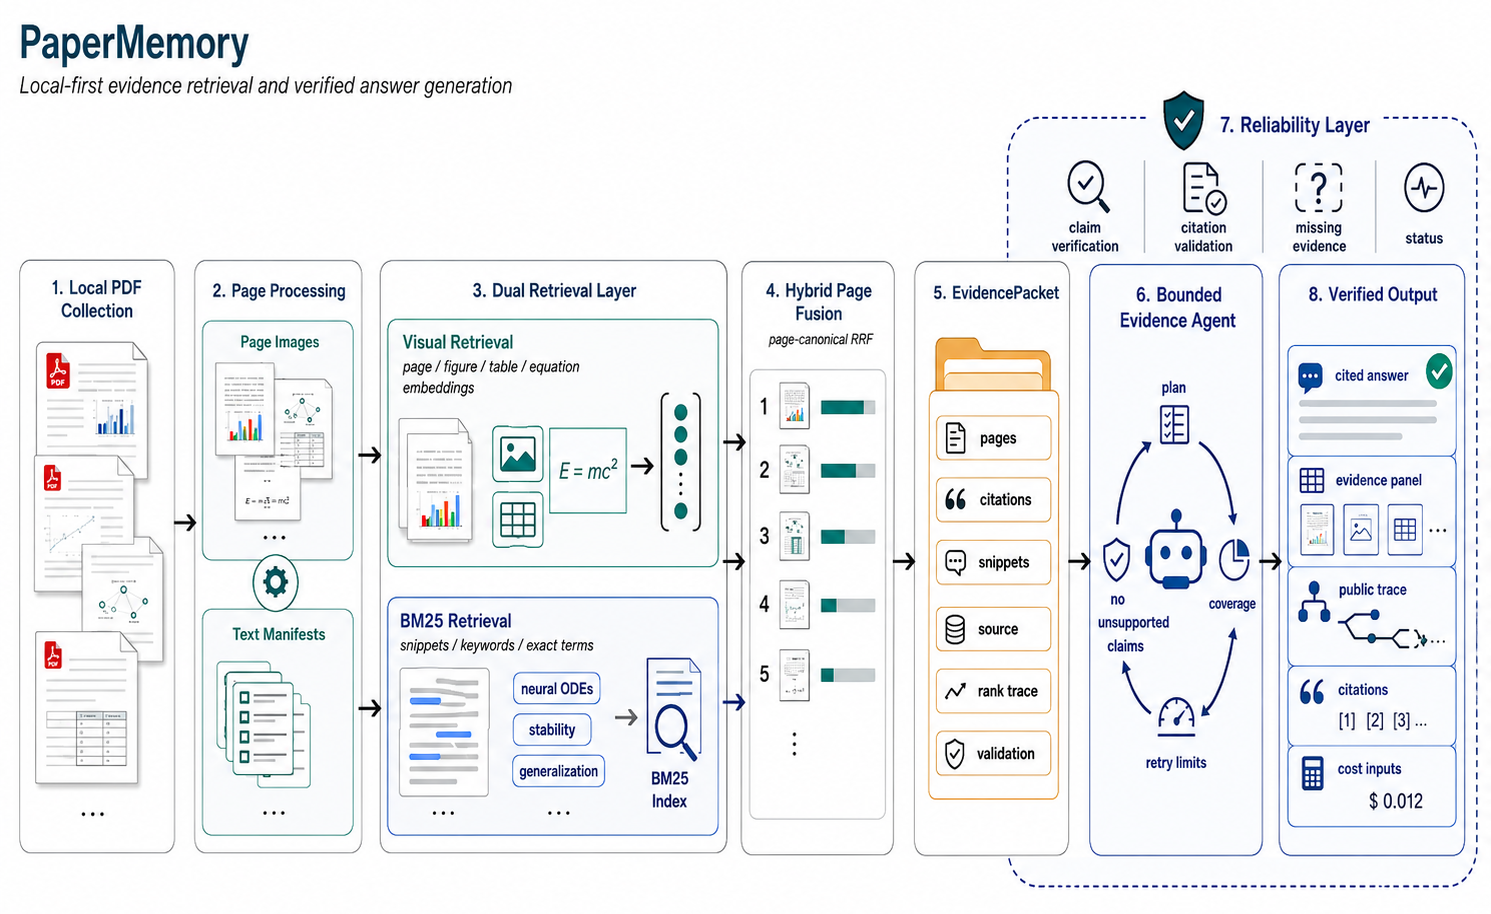
\includegraphics[width=\linewidth]{figures/papermemory_pipeline_figure1.png}
  \caption{PaperMemory pipeline with the reliability layer. The figure describes the report package over existing local artifacts; it does not add OCR, dense text retrieval, billing, or unrestricted agent actions.}
  \label{fig:pipeline}
\end{figure}


Retrieval has three implemented paths. The visual path retrieves page candidates from the page-image evidence surface. The BM25 path indexes the text manifests with $k_1=1.5$ and $b=0.75$. The hybrid path applies page-canonical reciprocal rank fusion with $k=60$, then collapses visual and text hits onto the same $(paper, page)$ unit. That canonical page key keeps the downstream citation grain stable even when the two retrievers disagree about score scale or rank source.

The EvidencePacket schema is the system boundary between retrieval and generation. A packet records the query, paper scope, accepted EvidenceUnits, accepted page citations, rank traces, source modality, validation state, and limits. The public packet excludes local filesystem paths and keeps stable evidence ids so that chat, trace logs, and report material can point back to the same page units \citep{paperMemoryEvidenceContract,paperMemoryChatPacket}. Generation is allowed to see packet context, but final citations are filtered back to accepted packet pages.

The reliability layer sits after packet construction and before the answer is treated as ready for the user. It plans evidence requirements from the question, checks whether the selected papers and claim types are covered, verifies answer claims against accepted evidence, and returns a visible \texttt{strong}, \texttt{partial}, or \texttt{insufficient} status. The status is a review signal, not a correctness certificate. It tells the user whether the packet supports the answer, where coverage is thin, and when the system should withhold or narrow a claim \citep{paperMemoryEvidenceReliability}.

This architecture also connects to the product cost model. Reliability checks add planner and verification calls when enabled, while disabled reliability mode avoids that extra work. The cost stress test therefore belongs in the architecture story as a deployment control: stronger grounding can be purchased with more model work when the task warrants it, and lighter runs remain available for lower-risk exploration \citep{paperMemoryCostBenefit}.

\section{Agentic Autonomy and Implementation Logic}

PaperMemory's autonomy is bounded and server-verified. The agent does not browse freely, execute arbitrary tools, or attempt a complete literature review. It follows a small state machine over the selected paper scope. Planner output is treated as an untrusted hint, then the server clamps pass budgets, query counts, and final evidence size before retrieval or answer generation can proceed.

\begin{table}[t]
  \caption{Bounded agent trace states. The agent can retry for missing evidence, but server checks keep actions inside the selected paper scope.}
  \label{tab:agent-trace-summary}
  \centering
  \small
  \setlength{\tabcolsep}{3pt}
  \begin{tabularx}{\linewidth}{p{0.16\linewidth}YYYY}
    \toprule
    State & Agent action & Tool or component & Stop or transition & Safety boundary \\
    \midrule
    Rewrite & Prepare a scoped retrieval query from the user turn. & Server planner hint. & Move to first retrieval. & Planner output is validated and budget-clamped. \\
    Retrieve & Retrieve page evidence for the selected papers. & Hybrid, visual, or BM25 retrieval. & Build accepted EvidencePacket units. & Retrieval stays inside active paper scope. \\
    Analyze & Compare packet evidence with required claims. & Requirement planner and coverage check. & Stop as \texttt{sufficient} or request targeted retry. & Missing evidence is recorded as a limit. \\
    Retry & Search for uncovered requirements. & Coverage-gated retrieval retry. & Add only new accepted page units. & Pass count and query count are fixed by server limits. \\
    Check & Check whether retry changed the packet. & Evidence delta and dedupe check. & Stop as \texttt{no\_new\_evidence} when delta is zero. & Repeated retrieval cannot loop forever. \\
    Answer & Generate with final packet context and cite accepted pages. & Chat service and claim verifier. & Return answer plus reliability status. & Citations outside packet pages are stripped. \\
    \bottomrule
  \end{tabularx}
\end{table}


The implemented loop starts with query rewrite. The system prepares a conversation-aware retrieval query, then runs first retrieval through the selected retrieval mode, normally hybrid for scoped chat. Evidence analysis inspects the accepted packet units and records missing requirements. If coverage is incomplete and the budget remains, the orchestrator issues a targeted second retrieval rather than answering immediately. The retry is coverage-gated: it must seek missing evidence, deduplicate accepted units, and report whether the new pass changed the packet.

Stop reasons are explicit. A \texttt{sufficient} trace can answer after the first pass when the packet covers the question. A \texttt{no\_new\_evidence} trace stops after a retry produces no new accepted units. The answer step then uses the final packet, strips citations that do not match accepted pages, and attaches the reliability status from the requirement, coverage, and claim-verification checks. A \texttt{partial} answer can still be useful when it says which part is supported. An \texttt{insufficient} answer asks the user to revise scope or add evidence instead of filling the gap with unsupported prose.

The live controlled run exercises the same boundary. The successful image-context chat returned HTTP 200, six evidence rows, six citations, three included evidence images, and a final \texttt{sufficient} stop reason. The missing-evidence chat used a bounded second retrieval and ended with \texttt{no\_new\_evidence}, while the answer stated that the evidence packet did not support the requested mitochondrial ribosome profiling claim. The prompt-injection-style page stayed evidence rather than instruction: the answer treated the page text as untrusted and did not reveal keys, execute tools, or alter citations \citep{paperMemoryAgentTraces,paperMemoryLiveLocalTest}.

\section{Baselines, Evaluation, and Technical Results}

The evaluation is a proof-of-capability package built from synthetic fixtures, deterministic regression tests, and a controlled local browser/API run. It is not a broad benchmark over scholarly PDFs. The synthetic retrieval suite has four papers, 12 pages, 12 golden questions, and three negative cases. The controlled local run used uploaded fixture PDFs and records UI flow, retrieval quality checks, bounded agent traces, and trust behavior. These artifacts support implementation claims, not claims about general corpus performance.

\begin{table}[t]
  \caption{Synthetic retrieval metrics from existing local artifacts. Higher is better for measured percentage columns.}
  \label{tab:retrieval-summary}
  \centering
  \small
  \setlength{\tabcolsep}{4pt}
  \begin{tabularx}{\linewidth}{YrrrrrY}
    \toprule
    Run & R@1 & R@3 & R@5 & Citation & Refusal & Boundary \\
    \midrule
    Keyword overlap baseline & 88.9\% & 100.0\% & 100.0\% & 100.0\% & 33.3\% & Same synthetic fixture; token overlap only, not LLM, BM25, VisRAG, or real corpus. \\
    Visual API baseline & 77.8\% & 100.0\% & 100.0\% & 100.0\% & 33.3\% & Synthetic smoke corpus; not a real PDF or real VisRAG result. \\
    BM25 text manifest & 88.9\% & 100.0\% & 100.0\% & 100.0\% & 100.0\% & Synthetic BM25-only text manifest fixture. \\
    Hybrid page fusion & 77.8\% & 100.0\% & 100.0\% & 100.0\% & 33.3\% & Synthetic page-canonical fusion; 27 units carry both traces. \\
    \bottomrule
  \end{tabularx}
\end{table}


The baseline comparison has four measured synthetic retrieval rows. The first row is a deliberately weak keyword-overlap baseline on the same 12 golden questions. It scores title and caption tokens, giving Recall@1 of 88.9\%, Recall@3 and Recall@5 of 100.0\%, citation-page correctness of 100.0\%, and retrieval-level refusal correctness of 33.3\%; it is executable but has no EvidencePacket, model reasoning, BM25 weighting, visual retrieval, or sufficiency gate \citep{paperMemoryKeywordBaseline}. The visual API baseline has Recall@1 of 77.8\%, Recall@3 and Recall@5 of 100.0\%, citation-page correctness of 100.0\%, and retrieval-level refusal correctness of 33.3\%. The BM25 text-manifest row improves refusal correctness to 100.0\% on the same synthetic setup, while preserving 100.0\% Recall@3, Recall@5, and citation-page correctness \citep{paperMemoryNode1,paperMemoryBm25Metrics}. GPT-only chat, Elicit, and Consensus remain qualitative market or workflow comparators rather than measured same-fixture retrieval baselines.

The hybrid page-fusion row should be read as provenance evidence. Its aggregate synthetic retrieval percentages match the visual baseline, but 27 returned units carry both visual and BM25 traces. That result confirms that page-canonical RRF can merge retriever evidence into a single packet unit without inventing a new citation grain \citep{paperMemoryHybridMetrics}. It does not show that hybrid retrieval is better on real paper collections.

The bounded evidence agent is evaluated through traces and regression behavior rather than Recall@k. The trace examples show accepted evidence ids, pass indexes, evidence deltas, stop reasons, and final packet limits. The controlled live run adds a more realistic smoke test: search and chat reached the local API, evidence cards appeared in the UI, citation chips were rendered, missing evidence stopped safely, and prompt-injection-style PDF text remained inside the evidence boundary. The main technical result is therefore narrower than a benchmark claim: the current implementation connects retrieval, EvidencePackets, bounded retries, reliability status, and UI evidence surfacing in a reproducible local workflow.

\section{Trust, Safety, and Robustness}
\label{sec:trust-robustness}

Trust in PaperMemory depends on visible failure behavior. A research assistant can be useful only if the user can see when the evidence packet is strong, partial, or insufficient. PaperMemory therefore treats every answer as a product of selected papers, accepted EvidenceUnits, packet limits, and a reliability status. The status is a review signal for the user. It is not a correctness certificate.

\begin{table}[t]
  \caption{Deterministic robustness package. Each case is a local regression fixture, not an adversarial benchmark.}
  \label{tab:robustness}
  \centering
  \small
  \setlength{\tabcolsep}{4pt}
  \begin{tabularx}{\linewidth}{YYY}
    \toprule
    Case & Expected behavior & Boundary \\
    \midrule
    Empty scope & Conversation-mode limit and paper-style citation stripping. & No proof that all unsupported prose is detected. \\
    Missing evidence & Partial packet with no accepted citations. & Covers empty accepted packets for known scope. \\
    No-new-evidence loop & Stop reason records zero evidence delta. & Page dedupe, not semantic novelty. \\
    Prompt-injection-like PDF text & PDF text remains untrusted evidence; unsafe planner hints are redacted. & Pattern-based deterministic phrases. \\
    Citation drift & Unsupported page labels are stripped. & Simple \texttt{paper\_id p.N} labels. \\
    Conflicting numeric evidence & Verification-needed limit is surfaced. & Numeric heuristic only. \\
    Low-text marker & Visual-first limit warns against invented missing text. & OCR remains future work. \\
    \bottomrule
  \end{tabularx}
\end{table}


The robustness package covers common ways a PDF-grounded assistant can fail. With an empty scope, PaperMemory enters conversation mode and strips paper-style citations because no selected paper evidence exists. With missing scoped evidence, the packet is partial, carries no accepted citations, and removes generated page labels that are not supported by the accepted packet. With repeated retrieval, a second pass that finds the same page stops with \texttt{no\_new\_evidence} rather than treating a duplicate as new support.

Prompt-injection-like PDF text is handled as untrusted evidence. The page text may appear inside the accepted evidence section, but planner prompts label it as evidence rather than instruction, extra action fields are rejected, and unsafe planner hints are removed from public traces. Citation drift is handled at serialization time: citations outside accepted packet pages, including unknown-paper labels, are stripped before the answer reaches the user. Conflicting numeric evidence adds a verification-needed limit instead of forcing a single value. Low-text, empty, or OCR-needed pages add a visual-first limit so the assistant does not invent text that was not extracted \citep{paperMemoryRobustness,paperMemoryFailureGallery}.

The reliability layer turns these cases into user-facing states. A \texttt{strong} answer has the planned evidence requirements covered by accepted pages. A \texttt{partial} answer can be useful, but the limits explain which evidence is missing or contested. An \texttt{insufficient} answer tells the user to change scope or add sources before treating the answer as paper-grounded. This is a practical review workflow for controlled local fixtures and live smoke tests. It is not a broad security result, an OCR result, or proof that every unsupported claim will be detected \citep{paperMemoryEvidenceReliability}.

\section{Commercial Stress Test}
\label{sec:commercial-stress}

The commercial question is whether evidence-packet work can save enough expert time to justify a paid workflow while keeping human verification in place. Node 9 models that question with:
\[
\text{net savings} = (h_m - h_p - h_v) r - c_a - c_l,
\]
where $h_m$ is manual work, $h_p$ is PaperMemory operation time, $h_v$ is human verification time, $r$ is a fully loaded hourly rate, $c_a$ is API or compute cost, and $c_l$ is a license allocation. The formula makes verification a cost, not an optional afterthought.

\begin{table}[t]
  \caption{Node 9 planning estimates under stated assumptions. API/compute cost is per scenario, and savings are net USD after operation, human verification, API/compute, and license assumptions.}
  \label{tab:cost-summary}
  \centering
  \small
  \setlength{\tabcolsep}{4pt}
  \begin{tabularx}{\linewidth}{Yrrrrr}
    \toprule
    Scenario & PDFs & API/compute & Low & Base & High \\
    \midrule
    10-PDF evidence packet & 10 & 0.19 & 52.35 & 183.70 & 334.76 \\
    30-PDF project evidence scan & 30 & 0.68 & 79.32 & 561.61 & 1175.45 \\
    Systematic-review pre-screening & 200 & 1.62 & -232.20 & 3423.86 & 7863.37 \\
    \bottomrule
  \end{tabularx}
\end{table}


The per-scenario API or compute cost is small in the current stress test: 0.19~USD for a 10-PDF evidence packet, 0.68~USD for a 30-PDF project evidence scan, and 1.62~USD for systematic-review pre-screening. Base-case net savings are 183.70~USD, 561.61~USD, and 3423.86~USD after operation, verification, API/compute, and license assumptions. The low case for systematic-review pre-screening is -232.20~USD, which matters. It shows that the value case can fail when verification time and deployment assumptions dominate.

\begin{table}[t]
  \caption{Proposed pricing tiers for a subscription experiment. The tiers avoid exact quotas until usage telemetry exists.}
  \label{tab:pricing-tiers}
  \centering
  \small
  \setlength{\tabcolsep}{4pt}
  \begin{tabularx}{\linewidth}{p{0.18\linewidth}YYY}
    \toprule
    Tier & Access model & Usage boundary & Human role \\
    \midrule
    Free BYOK & User provides an API key or local model path for limited local PDF groups; no included model spend. & BYOK usage remains outside PaperMemory-managed LLM spend, with local limits on groups and requests. & User verifies pages and manages their own model setup. \\
    10~USD/month & Provider-compliant PaperMemory API relay for users who prefer subscription access over BYOK-only setup. & Lower weekly managed-model cap, BYOK fallback above cap, rate limits, and fair-use controls. & User verifies cited pages before using claims in writing. \\
    20~USD/month & Provider-compliant API relay with a higher weekly managed-model boundary. & Higher weekly cap than the 10~USD tier, still with BYOK fallback, rate limits, and fair-use controls. & User remains responsible for expert judgment and final citation checks. \\
    \bottomrule
  \end{tabularx}
\end{table}

\begin{table}[t]
  \caption{Illustrative subscription stress test for provider-compliant managed-LLM API relay.}
  \label{tab:tier-economics}
  \centering
  \small
  \setlength{\tabcolsep}{3pt}
  \begin{tabularx}{\linewidth}{p{0.2\linewidth}YY}
    \toprule
    Tier & Modeled month & API cost and headroom \\
    \midrule
    Free BYOK & User-supplied model/key. & 0~USD PaperMemory model spend; 0~USD subscription revenue. \\
    10~USD/month & Four 10-PDF evidence-packet runs. & 4 $\times$ 0.19 = 0.76~USD; 9.24~USD before non-model costs. \\
    20~USD/month & Four 30-PDF evidence-scan runs. & 4 $\times$ 0.68 = 2.72~USD; 17.28~USD before non-model costs. \\
    Heavy-use guard & Eight 30-PDF evidence-scan runs. & 8 $\times$ 0.68 = 5.44~USD; 14.56~USD before non-model costs. \\
    \bottomrule
  \end{tabularx}
\end{table}


The interview signal supports a subscription experiment rather than a BYOK-only product. Seven of 10 interviewed postgraduate researchers preferred PaperMemory-provided API/model access through a monthly subscription. Table~\ref{tab:tier-economics} uses the 10-PDF and 30-PDF Node 9 API/compute estimates as illustrative managed-access stress cases, not production quotas or validated margins. The proposed packaging keeps the free tier as BYOK, then tests 10~USD/month and 20~USD/month managed-access tiers through compliant API relay. Those tiers are plausible only with weekly capped managed LLM usage, BYOK fallback, rate limits, or a fair-use policy. Exact quotas should come from usage telemetry, not this report.

The paid tiers bundle compliant managed LLM access support rather than unlimited inference. The weekly cap is the key margin control: once a user exceeds the managed allowance, the product can pause, ask the user to wait, or fall back to BYOK. This keeps the commercial claim tied to a bounded service design rather than an unlimited API subsidy or subscription-account arbitrage. The stress test does not prove paid conversion, retention, production margins, hosting cost, support cost, abuse cost, or legal cost. It also does not make PaperMemory a systematic-review replacement. The stronger commercial claim is narrower: under the current assumptions, API cost is not the main blocker for first-pass evidence gathering. The product risk sits in user adoption, verification effort, usage variance, and deployment licensing.

\section{Limitations, Ethics, and Reproducibility}
\label{sec:limitations-ethics-reproducibility}

The evaluation package is local and controlled. Retrieval metrics come from synthetic fixtures, not a broad scholarly PDF benchmark. The live test uses a small controlled corpus and includes one duplicate-upload pollution caveat. Text extraction is selectable-text only; low-text and scanned pages are flagged, but OCR is future work. The text path uses BM25 and page-canonical fusion, not dense semantic text retrieval. The reliability layer checks packet support for answer claims, but it does not establish exhaustive literature coverage.

The market evidence is also early. The interview sample has 10 postgraduate researchers, a mean conditional purchase likelihood of 4.2/5, and a 70\% preference for managed API/model access. The appendix records the questionnaire protocol, but the report uses only aggregate notes. Those numbers justify a product experiment, not a claim about paid adoption. The planned 10~USD/month and 20~USD/month tiers still need pricing tests, usage telemetry, support estimates, and churn data.

Ethically, PaperMemory should remain a first-pass assistant. It can reduce citation packaging work, but users still need to inspect cited pages before academic, medical, legal, or policy use. The local-first and BYOK options reduce some centralization risk, yet external model APIs may still receive prompts and evidence snippets if the user configures them. Public traces therefore avoid local paths and unsafe planner hints, and generated citations are constrained to accepted packet pages.

Reproducibility materials live under the active repository root \artifact{D:/codex/papermemory}. The older \artifact{D:/codex/llm\_paper\_assis/papermemory} path is now a junction to the same working tree. Appendix~\ref{app:reproducibility} records the branch, baseline environment, LaTeX command, and verification snapshots. Appendix~\ref{app:interview-validation} records the interview sample, questionnaire protocol, aggregate results, and limits. Appendix~\ref{app:robustness-cost} records the robustness gallery and cost assumptions. A separate three-minute demo video accompanies the submission; the report focuses on technical evidence, market proof, cost stress testing, and reproducibility.

\section{Conclusion}
\label{sec:conclusion}

PaperMemory addresses a concrete research workflow: turning a local PDF collection into cited first-pass evidence that a human can inspect. The current system is more than a chat box because it combines visual and text retrieval, page-canonical fusion, EvidencePackets, bounded evidence seeking, reliability status, and UI evidence surfacing. The strongest evidence is still local: synthetic retrieval fixtures, deterministic robustness tests, a controlled live run, early postgraduate interviews, and a cost stress test.

The next steps are practical rather than rhetorical. PaperMemory needs real local-corpus evaluation, OCR and dense text retrieval experiments, usage telemetry for the proposed subscription tiers, and clearer licensing decisions before deployment. Until then, the right claim is bounded: PaperMemory is a plausible local-first assistant for first-pass evidence gathering and citation packaging, with visible limits and human verification built into the workflow.

\begin{thebibliography}{35}

\bibitem[Artifex Software(2026)]{artifexLicensing}
Artifex Software.
\newblock Licensing.
\newblock \url{https://artifex.com/licensing}, source checked for Node 10.

\bibitem[BLS(2026a)]{blsManagementAnalysts}
U.S. Bureau of Labor Statistics.
\newblock Management Analysts.
\newblock \url{https://www.bls.gov/ooh/business-and-financial/management-analysts.htm}, Node 9 source snapshot 2026-06-24.

\bibitem[BLS(2026b)]{blsDataScientists}
U.S. Bureau of Labor Statistics.
\newblock Data Scientists.
\newblock \url{https://www.bls.gov/ooh/math/data-scientists.htm}, Node 9 source snapshot 2026-06-24.

\bibitem[BLS(2026c)]{blsMedicalScientists}
U.S. Bureau of Labor Statistics.
\newblock Medical Scientists.
\newblock \url{https://www.bls.gov/ooh/life-physical-and-social-science/medical-scientists.htm}, Node 9 source snapshot 2026-06-24.

\bibitem[Consensus(2026)]{consensusPricing}
Consensus.
\newblock Subscription Plans.
\newblock \url{https://help.consensus.app/en/articles/10087865-subscription-plans}, Node 9 market-context snapshot 2026-06-24.

\bibitem[Cormack et~al.(2009)]{cormack2009rrf}
Gordon V. Cormack, Charles L. A. Clarke, and Stefan Buettcher.
\newblock Reciprocal rank fusion outperforms Condorcet and individual rank learning methods.
\newblock In \emph{Proceedings of SIGIR}, pages 758--759, 2009.

\bibitem[Elicit(2026)]{elicitPricing}
Elicit.
\newblock Pricing.
\newblock \url{https://elicit.com/pricing}, Node 9 market-context snapshot 2026-06-24.

\bibitem[Faysse et~al.(2024)]{faysse2024colpali}
Manuel Faysse, Hugues Sibille, Tony Wu, Bilel Omrani, Gautier Viaud, Celine Hudelot, and Pierre Colombo.
\newblock ColPali: Efficient document retrieval with vision language models.
\newblock arXiv:2407.01449, 2024.

\bibitem[MuPDF(2026)]{mupdfLicense}
MuPDF.
\newblock MuPDF License.
\newblock \url{https://mupdf.readthedocs.io/en/1.27.0/license.html}, source checked for Node 10.

\bibitem[NeurIPS(2025a)]{neurips2025cfp}
NeurIPS.
\newblock NeurIPS 2025 Call for Papers.
\newblock \url{https://neurips.cc/Conferences/2025/CallForPapers}.

\bibitem[NeurIPS(2025b)]{neuripsChecklist2025}
NeurIPS.
\newblock NeurIPS Paper Checklist Guidelines.
\newblock \url{https://neurips.cc/public/guides/PaperChecklist}.

\bibitem[OpenAI(2026)]{openaiPricing2026}
OpenAI.
\newblock API pricing.
\newblock \url{https://openai.com/api/pricing/}, Node 9 source snapshot 2026-06-24.

\bibitem[PaperMemory(2026a)]{paperMemoryInterviewValidation}
PaperMemory local artifact.
\newblock Interview market validation.
\newblock \path{reports/final/results/interview_market_validation.md}.

\bibitem[PaperMemory(2026b)]{paperMemoryEvidenceReliability}
PaperMemory local artifact.
\newblock Evidence reliability layer.
\newblock \path{reports/final/results/evidence_reliability_layer.md}.

\bibitem[PaperMemory(2026c)]{paperMemoryLiveLocalTest}
PaperMemory local artifact.
\newblock Live local test log.
\newblock \path{reports/final/results/live_local_test_log.md}.

\bibitem[PaperMemory(2026d)]{paperMemoryNode0}
PaperMemory local artifact.
\newblock Node 0 reproducibility environment.
\newblock \path{reports/final/results/reproducibility_environment.md}.

\bibitem[PaperMemory(2026e)]{paperMemoryNode1}
PaperMemory local artifact.
\newblock Baseline retrieval metrics.
\newblock \path{reports/final/results/baseline_metrics.md}.

\bibitem[PaperMemory(2026o)]{paperMemoryKeywordBaseline}
PaperMemory local artifact.
\newblock Keyword overlap baseline metrics.
\newblock \path{reports/final/results/keyword_baseline_metrics.md}.

\bibitem[PaperMemory(2026f)]{paperMemoryEvidenceContract}
PaperMemory local artifact.
\newblock Evidence contract.
\newblock \path{reports/final/results/evidence_contract.md}.

\bibitem[PaperMemory(2026g)]{paperMemoryTextManifest}
PaperMemory local artifact.
\newblock Text manifest quality.
\newblock \path{reports/final/results/text_manifest_quality.md}.

\bibitem[PaperMemory(2026h)]{paperMemoryBm25Metrics}
PaperMemory local artifact.
\newblock BM25 text retrieval metrics.
\newblock \path{reports/final/results/bm25_metrics.md}.

\bibitem[PaperMemory(2026i)]{paperMemoryHybridMetrics}
PaperMemory local artifact.
\newblock Hybrid retrieval metrics.
\newblock \path{reports/final/results/hybrid_metrics.md}.

\bibitem[PaperMemory(2026j)]{paperMemoryChatPacket}
PaperMemory local artifact.
\newblock Node 6 verified chat and evidence UI.
\newblock \path{reports/final/results/chat_ui_packet.md}.

\bibitem[PaperMemory(2026k)]{paperMemoryAgentTraces}
PaperMemory local artifact.
\newblock Node 7 agent trace examples.
\newblock \path{reports/final/results/agent_trace_examples.md}.

\bibitem[PaperMemory(2026l)]{paperMemoryRobustness}
PaperMemory local artifact.
\newblock Node 8 robustness matrix.
\newblock \path{reports/final/results/robustness_matrix.md}.

\bibitem[PaperMemory(2026m)]{paperMemoryFailureGallery}
PaperMemory local artifact.
\newblock Node 8 failure gallery.
\newblock \path{reports/final/results/failure_gallery.md}.

\bibitem[PaperMemory(2026n)]{paperMemoryCostBenefit}
PaperMemory local artifact.
\newblock Node 9 cost-benefit stress test.
\newblock \path{reports/final/results/cost_benefit.md} and \path{reports/final/results/cost_benefit.csv}.

\bibitem[PyMuPDF(2026)]{pymupdfPypi}
PyMuPDF.
\newblock PyMuPDF project page.
\newblock \url{https://pypi.org/project/PyMuPDF/}, source checked for Node 10.

\bibitem[Robertson and Zaragoza(2009)]{robertson2009bm25}
Stephen Robertson and Hugo Zaragoza.
\newblock The probabilistic relevance framework: BM25 and beyond.
\newblock \emph{Foundations and Trends in Information Retrieval}, 3(4):333--389, 2009.

\bibitem[Yu et~al.(2024)]{yu2024visrag}
Shi Yu, Chaoyue Tang, Bokai Xu, Junbo Cui, Junhao Ran, Yukun Yan, Zhenghao Liu, Shuo Wang, Xu Han, Zhiyuan Liu, and Maosong Sun.
\newblock VisRAG: Vision-based retrieval-augmented generation on multi-modality documents.
\newblock arXiv:2410.10594, 2024.

\end{thebibliography}

\appendix
\section{Reproducibility Commands and Environment}
\label{app:reproducibility}

The active repository root is \artifact{D:/codex/papermemory}. The older \artifact{D:/codex/llm\_paper\_assis/papermemory} path is now a junction to this working tree. The Node 0 environment artifact records branch \artifact{codex/papermemory-evidence-agent}, baseline commit \artifact{6884d738df9d685bad4f5a673a7d13a7bc2fb691}, Python 3.12.7, Node.js v22.18.0, and npm 10.9.3 \citep{paperMemoryNode0}.

The final report package was compiled with the local LaTeX helper:
\begin{verbatim}
python "C:\Users\Miles CUI\.codex\plugins\cache\openai-bundled\latex\
0.2.2\scripts\compile_latex.py" D:\codex\papermemory\
reports\final\main.tex --json
\end{verbatim}

Earlier nodes recorded the following verification snapshots: Node 1 synthetic retrieval generation and JSON validation; Node 4 BM25 fixture generation; Node 5 hybrid fixture generation; Node 6 chat and evidence UI tests; Node 7 bounded orchestrator tests; Node 8 robustness tests with 11 focused passes; and Node 9 cost-model tests plus report regeneration. The canonical source artifacts for this report are stored under \artifact{reports/final/results/} and \artifact{eval/retrieval/results/}.

The package uses the official \artifact{neurips\_2025.sty} downloaded from the NeurIPS 2025 style link on the Call for Papers page \citep{neurips2025cfp}. The report uses anonymous submission style, not camera-ready or preprint mode.

\section{Interview Market Validation}
\label{app:interview-validation}

The market evidence comes from informal interviews with 10 postgraduate interviewees. The sample is small, so the results are treated as early intent evidence rather than paid adoption data.

\paragraph{Questionnaire protocol.}
Each interview used the same six prompts:
\begin{enumerate}
  \item What is your current research stage, and how often do you read PDFs?
  \item What is your current literature reading and citation-checking workflow?
  \item On a 1--5 scale, how likely would you be to pay if PaperMemory delivered local PDF ingestion, evidence-backed answers, visible page citations, bounded uncertainty, and smoother model access?
  \item Would you prefer BYOK/local-model setup or PaperMemory-provided LLM access through a subscription?
  \item Which packaging would you prefer: free BYOK with limited groups, 10~USD/month with a lower weekly managed-model limit, or 20~USD/month with a higher weekly managed-model limit?
  \item What risk would stop you from relying on the tool for research writing?
\end{enumerate}

\paragraph{Aggregate response.}
Across the 10 postgraduate interviewees, the mean conditional purchase likelihood was 4.2/5 if PaperMemory delivered the described workflow, and 70\% preferred PaperMemory-provided API/model access through a subscription over BYOK-only access. The report frames that paid option as provider-compliant API relay with caps, not consumer-account resale. The report does not claim participant-level raw data, paid conversion, retention, product-market fit, or production margins from this interview sample.

\begin{table}[h]
  \caption{Interview aggregate used in the market and revenue sections.}
  \label{tab:appendix-interview-validation}
  \centering
  \small
  \setlength{\tabcolsep}{4pt}
  \begin{tabularx}{\linewidth}{p{0.28\linewidth}p{0.18\linewidth}Y}
    \toprule
    Measure & Result & Report use \\
    \midrule
    Sample & 10 postgraduate researchers & Early postgraduate researcher signal, not a representative survey. \\
    Conditional purchase likelihood & 4.2 / 5 mean & Supports testing a paid evidence-workflow product if the promised functions are delivered. \\
    Managed API/model preference & 70\% & Supports adding monthly subscription tiers rather than offering BYOK only. \\
    Proposed tiers discussed in report & Free BYOK, 10~USD/month, 20~USD/month & Proposed packaging for stress testing, not launched billing. \\
    \bottomrule
  \end{tabularx}
\end{table}

\paragraph{How the report uses the result.}
The main report uses the interviews to justify a commercial experiment: a free BYOK tier for adoption, plus paid provider-compliant managed-access tiers for users who do not want to configure model keys. The result also explains why the cost model matters. If managed access is part of the product, model usage must have weekly caps, BYOK fallback above cap, rate limits, or fair-use controls.

\paragraph{Limitations.}
The interviews do not measure paid conversion, retention, referral, production revenue, support load, or willingness to keep paying after repeated use. The report therefore treats the numbers as market direction, not proof of demand.

\section{Full Metric Tables}
\label{app:full-metrics}

The retrieval summary in the main text is derived from generated CSV/Markdown artifacts under \artifact{eval/retrieval/results/}. The aggregate rows for the keyword overlap baseline, visual API baseline, BM25 baseline, and hybrid baseline are restated in Table~\ref{tab:appendix-retrieval}.

\begin{table}[h]
  \caption{Aggregate synthetic fixture metrics with corpus and path details.}
  \label{tab:appendix-retrieval}
  \centering
  \small
  \setlength{\tabcolsep}{4pt}
  \begin{tabularx}{\linewidth}{YYYY}
    \toprule
    Run & Setup & Metrics & Limits \\
    \midrule
    Keyword overlap baseline & Command recorded in the keyword metrics artifact. Scores title+caption pages by \texttt{TOKEN\_RE} token overlap on the same 12 golden questions. & R@1 88.9\%; R@3 100.0\%; R@5 100.0\%; citation-page 100.0\%; refusal 33.3\%. & Weak deterministic same-fixture comparator only; not LLM, BM25, VisRAG, real PDF, or real corpus evidence. \\
    Visual API baseline & Current FastAPI retrieval route over 4 synthetic papers, 12 pages, 12 golden questions, 3 refusal cases. & R@1 77.8\%; R@3 100.0\%; R@5 100.0\%; citation-page 100.0\%; refusal 33.3\%. & Not a real PDF, real local corpus, or real VisRAG evaluation. \\
    BM25 text manifest & Direct deterministic BM25 over synthetic TextManifest pages, $k_1=1.5$, $b=0.75$. & R@1 88.9\%; R@3 100.0\%; R@5 100.0\%; citation-page 100.0\%; refusal 100.0\%. & Synthetic text fixture only; no route, chat, hybrid, or OCR claim. \\
    Hybrid page fusion & Synthetic visual store plus synthetic text manifest, page-canonical RRF, $k=60$. & R@1 77.8\%; R@3 100.0\%; R@5 100.0\%; citation-page 100.0\%; refusal 33.3\%; 27 both-trace units. & Contract/provenance result, not a real-corpus improvement claim. \\
    \bottomrule
  \end{tabularx}
\end{table}

The hybrid artifact reports 37 units with visual traces, 27 with BM25 traces, 27 with both traces, 10 visual-only units, and 0 text-only units. This supports the page-canonical fusion claim: overlapping retriever evidence is collapsed into a shared evidence unit with rank traces instead of being exposed as duplicate citations.

\section{Robustness Failure Gallery and Cost Assumptions}
\label{app:robustness-cost}

The failure gallery records seven safe-failure snapshots: empty scope, missing scoped evidence, no-new-evidence loop, prompt-injection-like PDF text, citation drift, conflicting evidence, and low-text or scanned markers. The robustness matrix records 11 focused test passes for these fixtures. The expected behavior is containment and visible limits, not complete prevention of all possible prompt or citation failures. The supporting local artifacts are \artifact{robustness\_matrix.md} and \artifact{failure\_gallery.md} under \artifact{reports/final/results/}.

The cost model uses the stress-test formula:
\[
\text{net savings} = (h_m - h_p - h_v) r - c_a - c_l.
\]
Low-savings, base-savings, and high-savings cases vary manual and verification hours. Labor conversion uses annual wage divided by 2080 hours and multiplied by 1.35. Source values for OpenAI pricing, BLS wages, Elicit, and Consensus are a 2026-06-24 planning snapshot, so they should be refreshed before any customer-facing or investor-facing use.

\begin{table}[h]
  \caption{Cost-model assumptions from \artifact{cost\_benefit.csv}.}
  \label{tab:appendix-cost-assumptions}
  \centering
  \small
  \setlength{\tabcolsep}{4pt}
  \begin{tabularx}{\linewidth}{YrrrrY}
    \toprule
    Scenario & Runs & Input tok. & Cached tok. & Output tok. & Labor profile \\
    \midrule
    10-PDF evidence packet & 3 & 175000 & 25000 & 17500 & BLS management analysts, 65.68 USD/hr loaded. \\
    30-PDF project evidence scan & 6 & 690000 & 120000 & 54000 & BLS data scientists, 73.08 USD/hr loaded. \\
    Systematic-review pre-screening & 10 & 3500000 & 750000 & 250000 & BLS medical scientists, 65.29 USD/hr loaded. \\
    \bottomrule
  \end{tabularx}
\end{table}

PyMuPDF/MuPDF licensing remains unresolved for commercial deployment. The cost table therefore includes planning license allocations, but the paper does not convert those estimates into production margins. The cost spreadsheet and narrative are stored as \artifact{cost\_benefit.csv} and \artifact{cost\_benefit.md} under \artifact{reports/final/results/}.

The proposed 10~USD/month and 20~USD/month tiers are tier-economics assumptions rather than validated pricing telemetry. Weekly caps, BYOK fallback above cap, rate limits, and fair-use controls are product controls for provider-compliant managed LLM API relay; the report does not assume consumer-account pooling, unlimited inference, or production margins.


\section*{NeurIPS Paper Checklist}

This checklist follows the NeurIPS checklist guidance \citep{neuripsChecklist2025}. Answers are intentionally conservative.

\begin{enumerate}
\item \textbf{Claims.} \answerYes{} The abstract and introduction state that performance metrics are synthetic/local smoke evidence, and that interview evidence is early conditional intent rather than paid adoption.
\item \textbf{Limitations.} \answerYes{} Section~\ref{sec:limitations-ethics-reproducibility} and Appendix~\ref{app:robustness-cost} cover synthetic fixtures, no OCR, no dense text retrieval, no broad user study, and licensing risk.
\item \textbf{Theory.} \answerNA{} The paper does not introduce theorems or formal proofs.
\item \textbf{Reproducibility.} \answerYes{} Appendix~\ref{app:reproducibility} records commit, environment, commands, and local artifact paths.
\item \textbf{Datasets.} \answerYes{} The evaluation data are synthetic local fixtures described in the metrics artifacts. Appendix~\ref{app:interview-validation} describes the small interview sample used for market proof.
\item \textbf{Compute.} \answerYes{} The local Python, Node, npm, and LaTeX verification commands are recorded in the build notes and appendix.
\item \textbf{Ethics.} \answerYes{} Section 8 discusses human verification, privacy, prompt-boundary limits, and licensing risk.
\item \textbf{Broader impacts.} \answerYes{} The system can reduce first-pass citation labor and API setup friction, but misuse risk remains if users treat draft answers as verified scholarship.
\item \textbf{Safeguards.} \answerYes{} Deterministic guardrails are described for empty scope, missing evidence, prompt-injection-like PDF text, citation drift, conflicting evidence, and low-text markers.
\item \textbf{Licenses and assets.} \answerYes{} Local artifacts are listed, and PyMuPDF/MuPDF AGPL/commercial-license exposure is documented as a deployment risk.
\end{enumerate}

\end{document}
